% Provenance (never printed): cycle 3 / 6e "La planete Terre" (structure of
% the globe: crust, mantle, core); see sources/book1/PROVENANCE.md. Book 1,
% grade 6, chapter 4.
% Vocabulary guard: "magma" not before g7.2 ("molten rock"); P and S waves,
% Moho, core--mantle boundary and lithosphere belong to Book 2 (g11): the
% waves are told in prose, never defined; "seismometer" is defined in g7.3.
\chapter{Inside the Earth}\label{ch:g6:inside-the-earth}

In the far north-west of Russia, not far from the border with Norway, a metal cap is welded onto the ground among abandoned buildings. Under it, a hole only
about 23~centimetres wide goes straight down for more than 12~kilometres:
it is the deepest hole ever dug. Drilling it took about 20~years. The
drillers hoped to go deeper still, but at the bottom the \omterm{def:g3:stones-pebbles-sand:rock}{rock} was at about
180~degrees Celsius, almost twice as hot as expected: the heat bent the
drill bits and the pipes, and the work stopped in 1992. Yet the centre of
the Earth is more than \textbf{500 times} deeper than the bottom of that
hole. How can we know what lies down there?
% ledger: sciam:kola-depth, sciam:kola-180C, earth:Rmean

\begin{omfigure}
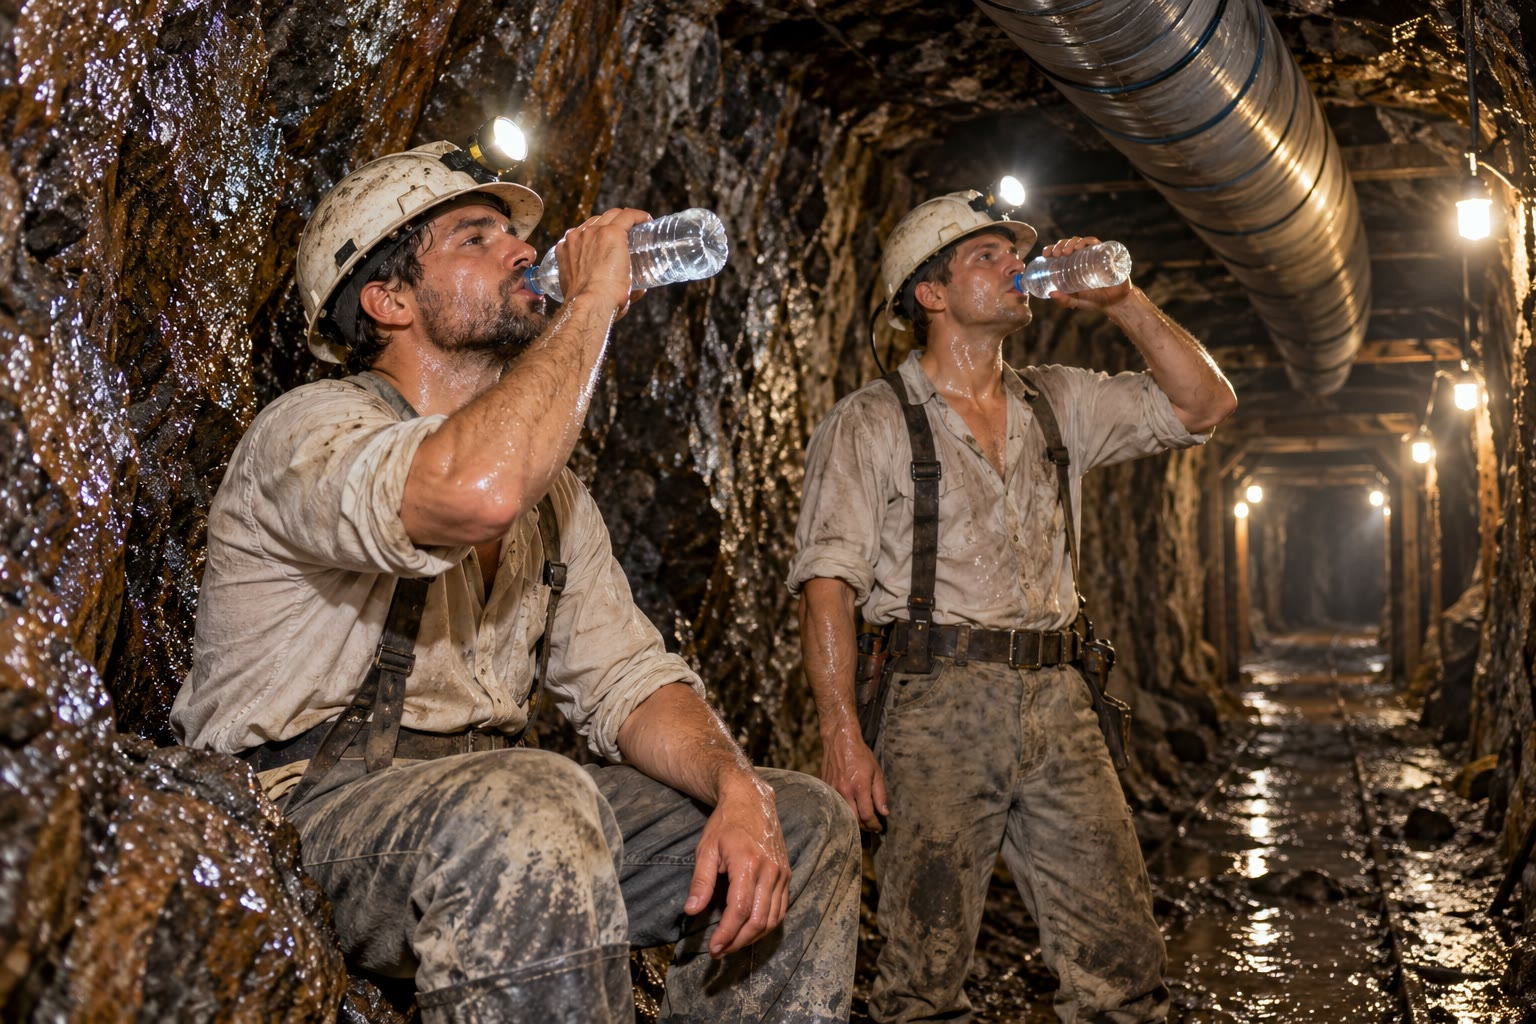
\includegraphics[width=0.62\linewidth]{images/book1/ai/g6-deep-mine.jpg}

{\small Miners take a drink in a hot gallery, kilometres under the ground.
(AI illustration.)}
\end{omfigure}

\begin{recall}
The Earth is a \omterm{def:g6:earth-a-planet:planet-types}{rocky planet}, a ball about 12\,742~km across: its radius,
from the surface to the centre, is about 6371~km
(\cref{ch:g6:earth-a-planet}). Its \omterm{def:g3:stones-pebbles-sand:rock}{rocks} belong to three families, igneous,
sedimentary and metamorphic (\cref{ch:g6:rocks-and-minerals}). At a
\omterm{def:g4:volcanoes-earthquakes-first-look:volcano}{volcano}, molten \omterm{def:g3:stones-pebbles-sand:rock}{rock} comes up from below and pours out as \omterm{def:g4:volcanoes-earthquakes-first-look:eruption}{lava}; in an
\omterm{def:g4:volcanoes-earthquakes-first-look:earthquake}{earthquake}, the ground shakes (\cref{ch:g4:volcanoes-earthquakes-first-look}).
\end{recall}
% ledger: earth:Rmean

\section{How deep have we been?}

People have long dug into the Earth, for water, stone
and metals. Two kinds of holes go the deepest.

\textbf{Mines.} The deepest mine in the world is a gold mine near
Johannesburg, in South Africa. Its galleries go down more than 4~km below
the surface. Down there, the \omterm{def:g3:stones-pebbles-sand:rock}{rock} walls reach about 60~degrees Celsius:
the mine is cooled by pumping down thousands of tonnes of ice mixed with
water, and by giant fans that blow air through the galleries.
% ledger: gwr:deepest-mine

\textbf{Boreholes.} A borehole is a narrow hole drilled from the surface
by a machine; nobody goes down it. The deepest one is the borehole of the
opening story, dug for science on the Kola Peninsula, in the north-west of Russia:
12\,262~metres, that is about 12.3~km.
% ledger: sciam:kola-depth

These depths look enormous. Compared with the size of the Earth, they are
tiny. The figure below shows them on one strip, next to the highest
\omterm{def:g1:landscapes-around-us:landform}{mountain}, Mount Everest (8849~m).
% ledger: tht:everest

\begin{omfigure}
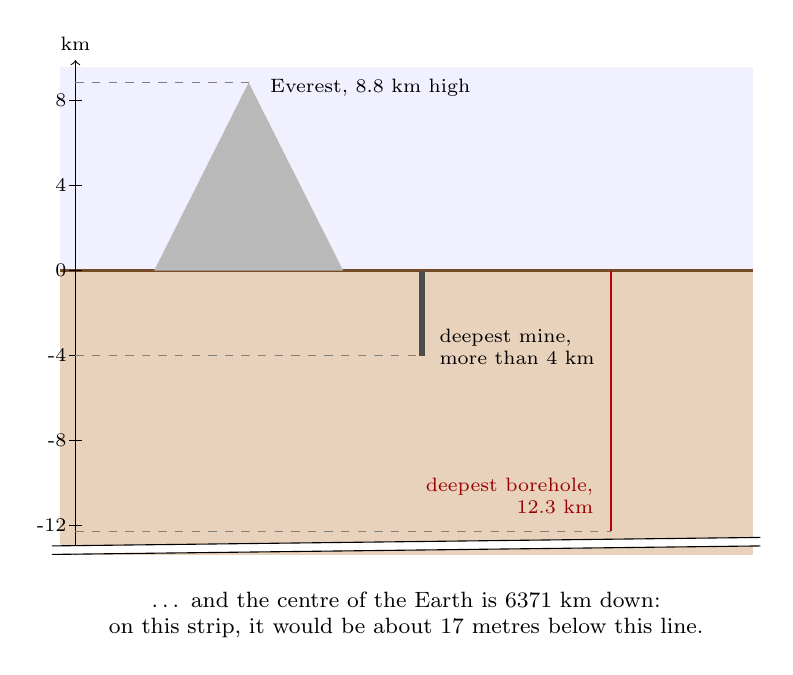
\begin{tikzpicture}[yscale=0.27, xscale=1]
  % sea-level ground and the sky
  \fill[blue!6] (-0.2,0) rectangle (8.6,9.6);
  \fill[brown!35] (-0.2,0) rectangle (8.6,-13.4);
  \draw[thick, brown!60!black] (-0.2,0) -- (8.6,0);
  % depth axis
  \draw[->] (0,-13.4) -- (0,9.9) node[above, font=\scriptsize] {km};
  \foreach \y in {-12,-8,-4,0,4,8} \draw (-0.08,\y) -- (0.08,\y) node[left=2pt, font=\scriptsize] {\y};
  % Everest
  \fill[gray!55] (1.0,0) -- (2.2,8.849) -- (3.4,0) -- cycle;
  \draw[dashed, gray] (0,8.849) -- (2.2,8.849);
  \node[font=\scriptsize, right] at (2.35,8.6) {Everest, 8.8~km high};
  % deepest mine
  \draw[line width=2.2pt, black!70] (4.4,0) -- (4.4,-4);
  \draw[dashed, gray] (0,-4) -- (4.4,-4);
  \node[font=\scriptsize, right, align=left] at (4.5,-3.6) {deepest mine,\\ more than 4~km};
  % Kola borehole
  \draw[line width=0.7pt, red!75!black] (6.8,0) -- (6.8,-12.262);
  \draw[dashed, gray] (0,-12.262) -- (6.8,-12.262);
  \node[font=\scriptsize, left, align=right, red!60!black] at (6.7,-10.6) {deepest borehole,\\ 12.3~km};
  % break and the centre
  \draw[white, line width=3pt] (-0.3,-13.15) -- (8.7,-12.75);
  \draw (-0.3,-13.35) -- (8.7,-12.95);
  \draw (-0.3,-12.95) -- (8.7,-12.55);
  \node[font=\footnotesize, align=center] at (4.2,-16.2) {\ldots\ and the centre of the Earth is 6371~km down:\\
     on this strip, it would be about 17~metres below this line.};
\end{tikzpicture}

{\small Heights and depths drawn to the same scale (1~cm for 3.7~km),
from \omterm{def:g4:world-physical-map:altitude}{sea level}. The break in the strip hides almost the whole way to the
centre.}
% ledger: tht:everest, gwr:deepest-mine, sciam:kola-depth, earth:Rmean
\end{omfigure}

\begin{method}[Comparing a depth with the radius of the Earth]\label{met:g6:inside-the-earth:percent}
\begin{enumerate}
  \item Write the depth and the radius in the same unit (kilometres).
  \item Divide the depth by the radius, then multiply by 100: this gives
        the depth as a percentage of the way to the centre.
  \item To say how many times deeper the centre is, divide the radius by
        the depth.
\end{enumerate}
\end{method}

\begin{example}[The deepest borehole]\label{ex:g6:inside-the-earth:kola}
The borehole is 12.3~km deep and the radius is 6371~km.
$12.3 \div 6371 \approx 0.0019$, and $0.0019 \times 100 = 0.19$: the
borehole went about \textbf{0.2~\%} of the way to the centre. The other way
round, $6371 \div 12.3 \approx 518$: the centre is more than 500~times
deeper than the bottom of the hole.

For the deepest mine, about 4~km: $4 \div 6371 \approx 0.0006$, that is
0.06~\%: three times less than the borehole.
% ledger: sciam:kola-depth, earth:Rmean, gwr:deepest-mine
\end{example}

So no one has ever seen, touched or sampled the deep inside of the Earth.
What we know of it comes from other clues, above all from the waves of
\omterm{def:g4:volcanoes-earthquakes-first-look:earthquake}{earthquakes} (section~\ref{sec:g6:inside-the-earth:waves}).

\section{Crust, mantle and core}

The Earth is built in layers, a little like a boiled egg: a thin brittle
shell, a thick ``white'', and a ``yolk'' in the middle.
% ledger: usgs:layers-egg

\begin{omfigure}
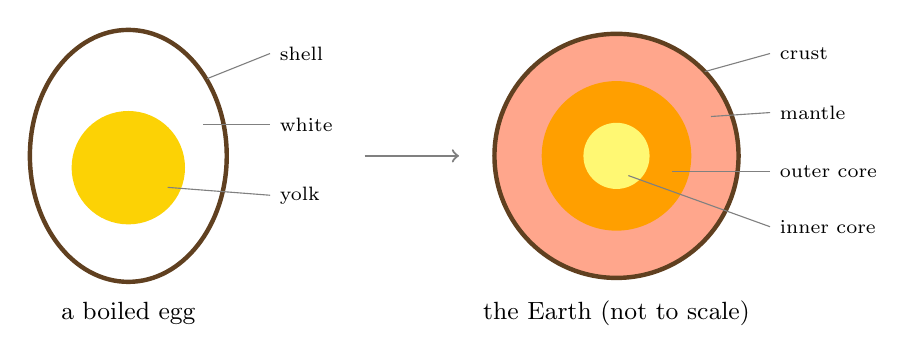
\begin{tikzpicture}
  % a boiled egg cut in half
  \begin{scope}
    \fill[white] (0,0) ellipse (1.25 and 1.6);
    \draw[brown!50!black, line width=1.6pt] (0,0) ellipse (1.25 and 1.6);
    \fill[yellow!70!orange] (0,-0.15) circle (0.72);
    \node[font=\scriptsize, anchor=west] (s) at (1.8,1.3) {shell};
    \draw[gray] (s.west) -- (1.0,0.98);
    \node[font=\scriptsize, anchor=west] (w) at (1.8,0.4) {white};
    \draw[gray] (w.west) -- (0.95,0.4);
    \node[font=\scriptsize, anchor=west] (y) at (1.8,-0.5) {yolk};
    \draw[gray] (y.west) -- (0.5,-0.4);
    \node[font=\small] at (0,-2.0) {a boiled egg};
  \end{scope}
  \draw[->, thick, gray] (3.0,0) -- (4.2,0);
  % the Earth, not to scale
  \begin{scope}[xshift=6.2cm]
    \fill[orange!45!red!45] (0,0) circle (1.55);
    \fill[orange!75!yellow] (0,0) circle (0.95);
    \fill[yellow!55] (0,0) circle (0.42);
    \draw[brown!50!black, line width=1.6pt] (0,0) circle (1.55);
    \node[font=\scriptsize, anchor=west] (c) at (1.95,1.3) {crust};
    \draw[gray] (c.west) -- (1.12,1.07);
    \node[font=\scriptsize, anchor=west] (m) at (1.95,0.55) {mantle};
    \draw[gray] (m.west) -- (1.2,0.5);
    \node[font=\scriptsize, anchor=west] (o) at (1.95,-0.2) {outer core};
    \draw[gray] (o.west) -- (0.7,-0.2);
    \node[font=\scriptsize, anchor=west] (i) at (1.95,-0.9) {inner core};
    \draw[gray] (i.west) -- (0.15,-0.25);
    \node[font=\small] at (0,-2.0) {the Earth (not to scale)};
  \end{scope}
\end{tikzpicture}

{\small The Earth compared with a boiled egg. Unlike the yolk, the \omterm{def:g6:inside-the-earth:layers}{core} has
two parts. In this drawing the \omterm{def:g6:inside-the-earth:layers}{crust} is shown much too thick; the drawing
to scale comes next.}
% ledger: usgs:layers-egg
\end{omfigure}

\begin{definition}[The layers of the Earth]\label{def:g6:inside-the-earth:layers}
The Earth is made of three main layers, from the surface to the centre:
\begin{itemize}
  \item the \emph{crust}\index{crust}, a thin outer layer of solid \omterm{def:g3:stones-pebbles-sand:rock}{rock}, a
        few kilometres to a few tens of kilometres thick;
  \item the \emph{mantle}\index{mantle}, a thick layer of hot, dense,
        solid \omterm{def:g3:stones-pebbles-sand:rock}{rock}, down to a depth of about 2900~km;
  \item the \emph{core}\index{core}, made of metal, mostly iron with some
        nickel, from about 2900~km down to the centre. The core has two
        parts: the \emph{outer core}\index{outer core}, which is liquid, and
        the \emph{inner core}\index{inner core}, a solid ball at the centre,
        about 1220~km in radius.
\end{itemize}
% ledger: usgs:layers-egg, usgs:crust-thickness, data:prem, earth:Rmean
\end{definition}

The drawing below shows the layers \emph{to scale}, with the boundaries
measured by \omterm{def:g4:volcanoes-earthquakes-first-look:earthquake}{earthquake} waves.

\begin{omfigure}
\pgfplotstableread{figdata/out/grade-6-earth_layers-disc.dat}\disctab
\pgfplotstablegetelem{0}{r_cm}\of\disctab \let\rE\pgfplotsretval
\pgfplotstablegetelem{1}{r_cm}\of\disctab \let\rOC\pgfplotsretval
\pgfplotstablegetelem{2}{r_cm}\of\disctab \let\rIC\pgfplotsretval
\begin{minipage}[c]{0.43\linewidth}\centering
\begin{tikzpicture}
  \fill[orange!45!red!45] (0,0) circle (\rE cm);
  \fill[orange!75!yellow] (0,0) circle (\rOC cm);
  \fill[yellow!55] (0,0) circle (\rIC cm);
  \draw[brown!50!black, line width=0.45pt] (0,0) circle (\rE cm);
  
  \draw[gray, thin] (-0.25,\rE) rectangle (0.25,\rE-0.12);
  
  \node[font=\scriptsize, align=center, inner sep=0pt] at (0,0) {inner\\ core};
  \node[font=\scriptsize, align=center] at (0,1.03) {outer\\ core};
  \node[font=\scriptsize] at (0,2.12) {mantle};
  \draw[<-, font=\scriptsize] (1.98,1.98) -- (2.3,2.75) node[above, align=center] {crust\\ (a hairline)};
\end{tikzpicture}
\end{minipage}\hfill
\begin{minipage}[c]{0.55\linewidth}\centering
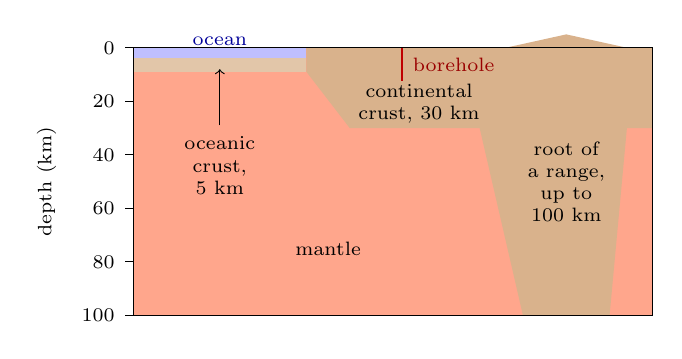
\begin{tikzpicture}[yscale=0.034, xscale=0.55]
  % the top 100 km enlarged: ocean on the left, continent and a range on the right
  \fill[orange!45!red!45] (0,0) rectangle (12,-100);
  \fill[blue!25] (0,0) rectangle (4,-4);
  \fill[brown!45] (0,-4) rectangle (4,-9);                 % oceanic crust 5 km
  \fill[brown!60] (4,0) -- (4,-9) -- (5,-30) -- (8,-30) -- (9,-100) -- (11,-100) -- (11.4,-30) -- (12,-30) -- (12,0) -- cycle;
  \fill[brown!60] (8.6,0) -- (10,5) -- (11.4,0) -- cycle;   % the range (not to scale above ground)
  \draw[red!75!black, line width=0.8pt] (6.2,0) -- (6.2,-12.262);
  \draw[thin] (0,0) rectangle (12,-100);
  \foreach \y in {0,-20,-40,-60,-80,-100} \draw (0,\y) -- (-0.2,\y) node[left, font=\scriptsize] {\pgfmathparse{-\y}\pgfmathprintnumber{\pgfmathresult}};
  \node[font=\scriptsize, rotate=90] at (-2.0,-50) {depth (km)};
  \node[font=\scriptsize, align=center] at (2,-44) {oceanic\\ crust,\\ 5~km};
  \draw[->, thin] (2,-29) -- (2,-8);
  \node[font=\scriptsize, align=center] at (6.6,-21) {continental\\ crust, 30~km};
  \node[font=\scriptsize, align=center] at (10.0,-50) {root of\\ a range,\\ up to\\ 100~km};
  \node[font=\scriptsize, align=center, red!60!black] at (7.4,-6.5) {borehole};
  \node[font=\scriptsize] at (4.5,-75) {mantle};
  \node[font=\scriptsize, blue!60!black] at (2,2.5) {ocean};
\end{tikzpicture}
\end{minipage}

\smallskip
{\small Left: the Earth cut open, to scale; the small grey box at the top
marks the part enlarged on the right. Right: the top 100~km, enlarged about
60~times: thin \omterm{def:g6:inside-the-earth:layers}{crust} under the \omterm{def:g2:water-on-earth:ocean}{oceans}, thicker \omterm{def:g6:inside-the-earth:layers}{crust} under the \omterm{def:g3:continents-and-oceans:continent}{continents},
thickest under high \omterm{def:g4:world-physical-map:range}{mountain ranges}; the record borehole in red.}
% ledger: data:prem, earth:Rmean, usgs:crust-thickness, sciam:kola-depth (figdata/grade-6/earth_layers.py)
\end{omfigure}

\begin{center}\small
\begin{tabular}{|l|c|c|c|l|}
\hline
\textbf{layer} & \textbf{from (km)} & \textbf{to (km)} & \textbf{thickness (km)} & \textbf{made of} \\
\hline
\omterm{def:g6:inside-the-earth:layers}{crust} & 0 & 5 to 100 & 5 to 100 & solid \omterm{def:g3:stones-pebbles-sand:rock}{rock} \\
\omterm{def:g6:inside-the-earth:layers}{mantle} & bottom of the \omterm{def:g6:inside-the-earth:layers}{crust} & 2891 & about 2860 & solid \omterm{def:g3:stones-pebbles-sand:rock}{rock}, very hot \\
\omterm{def:g6:inside-the-earth:layers}{outer core} & 2891 & 5150 & about 2260 & liquid metal \\
\omterm{def:g6:inside-the-earth:layers}{inner core} & 5150 & 6371 (centre) & about 1220 & solid metal \\
\hline
\end{tabular}
\end{center}
% ledger: data:prem, usgs:crust-thickness, usgs:layers-egg, earth:Rmean (figdata/grade-6/earth_layers.py, main table)

\textbf{The \omterm{def:g6:inside-the-earth:layers}{crust}} is the only layer we can walk on and dig into. It is very
thin compared with the others: under the \omterm{def:g2:water-on-earth:ocean}{oceans}, it is only about 5~km
thick; under the \omterm{def:g3:continents-and-oceans:continent}{continents}, about 30~km on average; under high \omterm{def:g4:world-physical-map:range}{mountain
ranges} such as the Alps, its base can be as deep as 100~km, like the root
of a tooth. Even the record borehole, 12.3~km deep, went less than half way through an average continental \omterm{def:g6:inside-the-earth:layers}{crust}. On the drawing to scale, the \omterm{def:g6:inside-the-earth:layers}{crust}
is thinner than the line around the disc.
% ledger: usgs:crust-thickness, sciam:kola-depth

\textbf{The \omterm{def:g6:inside-the-earth:layers}{mantle}} is the thickest layer: it goes from the base of the
\omterm{def:g6:inside-the-earth:layers}{crust} down to 2891~km, about 45~\% of the way to the centre. Its \omterm{def:g3:stones-pebbles-sand:rock}{rock} is
solid, but very hot and denser than the \omterm{def:g3:stones-pebbles-sand:rock}{rock} of the \omterm{def:g6:inside-the-earth:layers}{crust}. Over millions of
years, the hot \omterm{def:g3:stones-pebbles-sand:rock}{rock} of part of the \omterm{def:g6:inside-the-earth:layers}{mantle} can creep very slowly, like a
very stiff paste.
% ledger: data:prem, usgs:layers-egg, usgs:lithosphere-80km

\textbf{The \omterm{def:g6:inside-the-earth:layers}{core}} begins at 2891~km and goes down to the centre. It is
made not of \omterm{def:g3:stones-pebbles-sand:rock}{rock} but of metal: an alloy of iron and nickel, nearly twice as
dense as the \omterm{def:g6:inside-the-earth:layers}{mantle}. Its outer part is \emph{liquid}: an \omterm{def:g2:water-on-earth:ocean}{ocean} of molten
metal more than 2000~km deep. Its inner part, from 5150~km down to the
centre, is a \emph{solid} ball of metal, about 1220~km in radius: about 70~\% as wide as the Moon. As the Earth turns, the liquid metal of the
\omterm{def:g6:inside-the-earth:layers}{outer core} moves, and this motion makes the Earth's magnetic field, the
one that turns a compass needle.
% ledger: data:prem, usgs:layers-egg, earth:Rmean, planet:Moon.diameter

The deeper, the denser. Water has a density of 1~gram per cubic
centimetre: the \omterm{def:g3:stones-pebbles-sand:rock}{rock} of the \omterm{def:g6:inside-the-earth:layers}{crust} is between 2.6 and 2.9 times as dense,
the \omterm{def:g3:stones-pebbles-sand:rock}{rock} at the bottom of the \omterm{def:g6:inside-the-earth:layers}{mantle} more than 5~times, and the metal at
the centre about 13~times (see the graph below). The heaviest materials are at the centre and the lightest on top: the Earth is sorted, from the light \omterm{def:g6:inside-the-earth:layers}{crust} to the heavy metal \omterm{def:g6:inside-the-earth:layers}{core}.
% ledger: data:prem


\begin{omfigure}
\begin{tikzpicture}
  \begin{axis}[omrecord, width=0.86\linewidth, height=5.4cm,
      xmin=0, xmax=6371, ymin=0, ymax=14,
      xlabel={depth below the surface (km)},
      ylabel={density (g per cm$^3$)},
      xtick={0,1000,2000,3000,4000,5000,6000},
      scaled x ticks=false, x tick label style={/pgf/number format/1000 sep={}},
      clip=false]
    \fill[orange!45!red!20] (axis cs:24.4,0) rectangle (axis cs:2891,14);
    \fill[orange!75!yellow!35] (axis cs:2891,0) rectangle (axis cs:5149.5,14);
    \fill[yellow!30] (axis cs:5149.5,0) rectangle (axis cs:6371,14);
    \addplot[very thick, black] table[x=depth_km, y=rho] {figdata/out/grade-6-earth_layers-profile.dat};
    \node[font=\scriptsize] at (axis cs:1450,12.5) {mantle};
    \node[font=\scriptsize] at (axis cs:4020,4.5) {outer core};
    \node[font=\scriptsize] at (axis cs:5760,4.5) {inner core};
    \node[font=\scriptsize, align=left, anchor=west] at (axis cs:80,1.4) {crust: 2.6 to 2.9};
  \end{axis}
\end{tikzpicture}

{\small How dense the Earth is at each depth, from a reference model built
from \omterm{def:g4:volcanoes-earthquakes-first-look:earthquake}{earthquake} measurements. The density jumps from about 5.6 to about
9.9~g per cm$^3$ where the \omterm{def:g3:stones-pebbles-sand:rock}{rock} of the \omterm{def:g6:inside-the-earth:layers}{mantle} gives way to the metal of the
\omterm{def:g6:inside-the-earth:layers}{core}.}
% ledger: data:prem (figdata/grade-6/earth_layers.py, part profile)
\end{omfigure}

\begin{inthelab}[Layers in a glass (in class, with the teacher)]
The teacher pours, slowly and one after the other, into a tall glass:
some honey, some water coloured with a drop of ink, and some cooking oil.
Whatever the order of pouring, after a moment the honey lies at the
bottom, the water in the middle and the oil on top: each liquid settles
below the lighter ones and above the denser ones. Shaken, the glass turns
cloudy; left alone, it sorts itself again. The Earth is layered in the same way: the densest material, the metal of the \omterm{def:g6:inside-the-earth:layers}{core}, is at the centre, and the lightest \omterm{def:g3:stones-pebbles-sand:rock}{rock} is on top.
\end{inthelab}


\begin{remark}[How thin is the crust?]\label{rem:g6:inside-the-earth:thin-crust}
On a school \omterm{def:g3:continents-and-oceans:globe}{globe} 30~cm across, the continental \omterm{def:g6:inside-the-earth:layers}{crust} (30~km) would be
about 0.7~millimetre thick, and the oceanic \omterm{def:g6:inside-the-earth:layers}{crust} (5~km) about the
thickness of a sheet of paper. The \omterm{def:g6:inside-the-earth:layers}{crust} is less than half of one
percent of the radius: $30 \div 6371 \approx 0.0047$, that is 0.47~\%.
% ledger: usgs:crust-thickness, earth:Rmean
\end{remark}

\section{How earthquake waves tell us the rest}\label{sec:g6:inside-the-earth:waves}

If no one has been deeper than 12~km, how can we draw the \omterm{def:g6:inside-the-earth:layers}{core}? The answer
comes from \omterm{def:g4:volcanoes-earthquakes-first-look:earthquake}{earthquakes}. When an \omterm{def:g4:volcanoes-earthquakes-first-look:earthquake}{earthquake} shakes the ground, waves leave
it in all directions and travel \emph{through} the whole Earth, like the
sound of a knock travels through a wall. Instruments in many places around the world record when each wave arrives (you will meet them in
\cref{ch:g7:earthquakes}).
% ledger: data:prem

The waves do not travel at the same speed in every material. When they
reach the boundary between two layers, their speed changes suddenly: some
waves bounce back, others bend as they cross, a little like light entering
water. By timing the waves of many \omterm{def:g4:volcanoes-earthquakes-first-look:earthquake}{earthquakes}, at stations all around the \omterm{def:g3:continents-and-oceans:globe}{globe}, scientists have found where these boundaries are, and
which layers are solid or liquid. Seismologists call the two main kinds of
waves \emph{P waves} (the faster ones, which push and pull the \omterm{def:g3:stones-pebbles-sand:rock}{rock}) and
\emph{S waves} (the slower ones, which shake it from side to side); later
volumes study them closely. The S waves have one remarkable property: they
cannot travel through a liquid.

\begin{omfigure}
\begin{tikzpicture}
  \begin{axis}[omrecord, width=0.86\linewidth, height=5.4cm,
      xmin=0, xmax=6371, ymin=0, ymax=14.5,
      xlabel={depth below the surface (km)},
      ylabel={wave speed (km per second)},
      xtick={0,1000,2000,3000,4000,5000,6000},
      scaled x ticks=false, x tick label style={/pgf/number format/1000 sep={}},
      clip=false]
    \fill[orange!45!red!20] (axis cs:24.4,0) rectangle (axis cs:2891,14.5);
    \fill[orange!75!yellow!35] (axis cs:2891,0) rectangle (axis cs:5149.5,14.5);
    \fill[yellow!30] (axis cs:5149.5,0) rectangle (axis cs:6371,14.5);
    \addplot[very thick, blue!70!black] table[x=depth_km, y=vp] {figdata/out/grade-6-earth_layers-profile.dat};
    \addplot[very thick, red!75!black] table[x=depth_km, y=vs] {figdata/out/grade-6-earth_layers-profile.dat};
    \node[font=\scriptsize, blue!70!black, anchor=south] at (axis cs:1300,12.9) {P waves (faster)};
    \node[font=\scriptsize, red!75!black, anchor=north] at (axis cs:1500,6.1) {S waves (slower)};
    \node[font=\scriptsize, red!75!black, align=center, fill=white, fill opacity=0.8, text opacity=1] at (axis cs:4020,1.9) {S waves: 0\\ (liquid)};
    \node[font=\scriptsize] at (axis cs:4020,13.6) {outer core};
    \node[font=\scriptsize] at (axis cs:5760,13.6) {inner core};
    \node[font=\scriptsize] at (axis cs:1450,1.5) {mantle};
  \end{axis}
\end{tikzpicture}

{\small The speed of the two kinds of \omterm{def:g4:volcanoes-earthquakes-first-look:earthquake}{earthquake} waves at each depth, in
the same reference model. In the \omterm{def:g6:inside-the-earth:layers}{outer core} the S waves stop: their speed
is zero, because the \omterm{def:g6:inside-the-earth:layers}{outer core} is liquid.}
% ledger: data:prem (figdata/grade-6/earth_layers.py, part profile)
\end{omfigure}

Reading the graph from left to right: in the \omterm{def:g6:inside-the-earth:layers}{mantle}, both kinds of waves
go faster and faster with depth. At 2891~km, the S waves disappear and the
P waves suddenly slow down: this is the top of the liquid \omterm{def:g6:inside-the-earth:layers}{outer core}. At
5150~km, the P waves speed up again and S waves exist once more: this is
the solid \omterm{def:g6:inside-the-earth:layers}{inner core}.
% ledger: data:prem

\begin{history}[Inge Lehmann and the inner core]
\begin{minipage}[c]{0.72\linewidth}
In the early 1930s, seismologists thought that the Earth had two layers: a solid \omterm{def:g6:inside-the-earth:layers}{mantle} around a liquid \omterm{def:g6:inside-the-earth:layers}{core}. The Danish seismologist Inge Lehmann studied the waves of a
strong \omterm{def:g4:volcanoes-earthquakes-first-look:earthquake}{earthquake} that struck New Zealand in 1929, recorded at stations
far away. Some waves arrived where, for a fully liquid \omterm{def:g6:inside-the-earth:layers}{core}, they should
not have arrived at all. In an article of 1936, simply called ``P\,$'$'',
she proposed an explanation: inside the liquid \omterm{def:g6:inside-the-earth:layers}{core} there is a smaller
\emph{solid \omterm{def:g6:inside-the-earth:layers}{inner core}}, which sends these waves back. She wrote modestly
that the data were ``quite insufficient'' to be sure, but that the
interpretation ``seems possible'', and she asked other researchers to test
it. They did, and today the solid \omterm{def:g6:inside-the-earth:layers}{inner core} is part of every reference model of the Earth, like the one used in the graphs of this chapter.
% ledger: nbi:lehmann-1936
\end{minipage}\hfill
\begin{minipage}[c]{0.24\linewidth}\centering
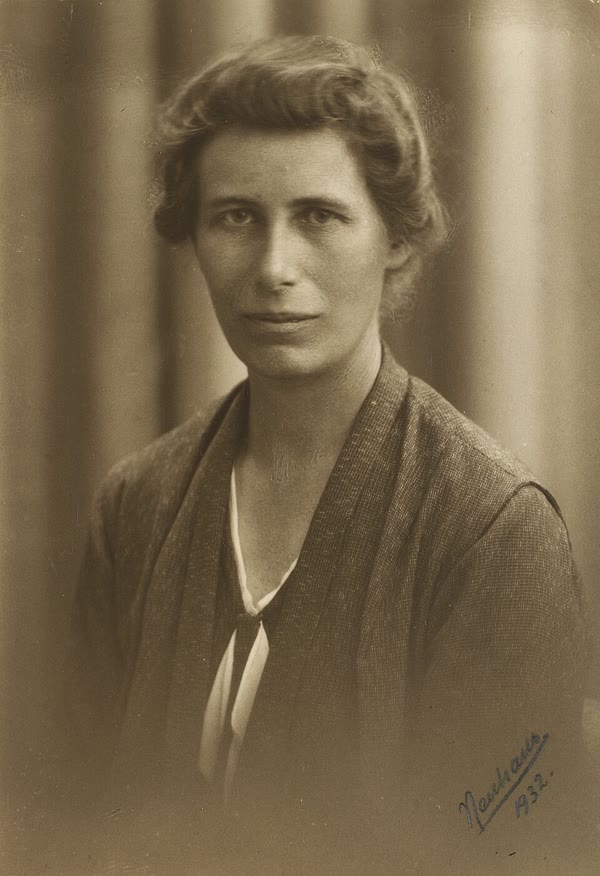
\includegraphics[width=\linewidth]{images/book1/g6-inge-lehmann.jpg}\\[2pt]
{\footnotesize Inge Lehmann in 1932. (Photo: Even Neuhaus, public domain,
via Wikimedia Commons.)}
% ledger: commons:inge-lehmann
\end{minipage}
\end{history}

\section{The deeper, the hotter}

Every deep mine and every deep borehole shows the same thing: the deeper
you go, the hotter the \omterm{def:g3:stones-pebbles-sand:rock}{rock}. In the deepest mine, the \omterm{def:g3:stones-pebbles-sand:rock}{rock} walls reach
about 60~degrees Celsius, more than 4~km down; at the bottom of the record
borehole, 12.3~km down, the \omterm{def:g3:stones-pebbles-sand:rock}{rock} was at about 180~degrees.
% ledger: gwr:deepest-mine, sciam:kola-180C

Near the surface, the temperature rises at a fairly steady rate. In the
United States, scientists gathered the measurements of 284 drill holes,
most of them deeper than 600~m. On average, the temperature rose by
\textbf{29~degrees for each kilometre} of depth: about 25~degrees per
kilometre in the east of the country and 34 in the west. But the rate
varies a lot from place to place: in those holes, it went from 6 to
69~degrees per kilometre.
% ledger: usgs:gradient-29

\begin{omfigure}
\begin{tikzpicture}
  \begin{axis}[omrecord, omdepth, width=0.78\linewidth, height=5.6cm,
      xmin=0, xmax=160, ymin=0, ymax=2,
      xlabel={temperature of the rock ($^\circ$C)},
      ylabel={depth (km)},
      ytick={0,0.5,1,1.5,2},
      yticklabel style={/pgf/number format/fixed},
      legend pos=north east, legend cell align=left,
            legend style={font=\scriptsize},
      clip=false]
    \addplot[forget plot, name path=lo, thin, gray] table[x=t_low, y=depth_km] {figdata/out/grade-6-earth_layers-geotherm.dat};
    \addplot[forget plot, name path=hi, thin, gray] table[x=t_high, y=depth_km] {figdata/out/grade-6-earth_layers-geotherm.dat};
    \addplot[forget plot, gray!20] fill between[of=lo and hi];
    \addplot[forget plot, thick, blue!70!black] table[x=t_east, y=depth_km] {figdata/out/grade-6-earth_layers-geotherm.dat};
    \addplot[forget plot, very thick, black] table[x=t_mean, y=depth_km] {figdata/out/grade-6-earth_layers-geotherm.dat};
    \addplot[forget plot, thick, red!75!black] table[x=t_west, y=depth_km] {figdata/out/grade-6-earth_layers-geotherm.dat};
    \addlegendimage{area legend, fill=gray!20, draw=gray}
    \addlegendentry{6 to 69 $^\circ$C per km: all the holes}
    \addlegendimage{thick, blue!70!black}\addlegendentry{25 $^\circ$C per km: east}
    \addlegendimage{very thick, black}\addlegendentry{29 $^\circ$C per km: average}
    \addlegendimage{thick, red!75!black}\addlegendentry{34 $^\circ$C per km: west}
  \end{axis}
\end{tikzpicture}

{\small Temperature against depth (downward) for a ground starting at
15~$^\circ$C, at the average rate (29, black), the eastern and western
averages (25 and 34) and the whole measured range (6 to 69, grey band). The
measurements reach about 2~km.}
% ledger: usgs:gradient-29, planet:Earth.Tmean (figdata/grade-6/earth_layers.py, part geotherm)
\end{omfigure}

\begin{method}[Temperature at a depth]\label{met:g6:inside-the-earth:temperature}
\begin{enumerate}
  \item Take the temperature of the ground near the surface.
  \item Multiply the depth, in kilometres, by the rate, in degrees per
        kilometre: this is how much warmer it gets.
  \item Add the two. Use it only over the range where the rate was
        measured: a few kilometres.
\end{enumerate}
\end{method}

\begin{example}[Two kilometres down]\label{ex:g6:inside-the-earth:two-km}
The ground is at 15~$^\circ$C and the rate is 29~degrees per kilometre.
At 2~km: $2 \times 29 = 58$ degrees warmer, so $15 + 58 = 73~^\circ$C:
hotter than the hottest bath, and already far too hot to touch.
% ledger: usgs:gradient-29, planet:Earth.Tmean
\end{example}

Can the same rate be used all the way to the centre? No. At 29~degrees per
kilometre, the centre would be at about 185\,000~degrees, which is
impossible: the rate measured in the first kilometres does not hold deep down, where the rise must be much slower. Scientists estimate the temperature
of the \omterm{def:g6:inside-the-earth:layers}{core} in another way: in the laboratory, they squeeze tiny grains of
iron between two diamonds, to millions of times the pressure of the air,
and heat them with lasers until they melt. In this way, they found that
at the edge of the solid \omterm{def:g6:inside-the-earth:layers}{inner core} the temperature is about
\textbf{6000~degrees Celsius}, and yet the iron of the \omterm{def:g6:inside-the-earth:layers}{inner core} stays solid, because the pressure there, about
3.3~million times the pressure of the air, keeps it from melting.
% ledger: esrf:core-6000C, usgs:gradient-29

\begin{remark}[Hot, and still solid]\label{rem:g6:inside-the-earth:pressure}
Squeezing a substance hard makes it melt only at a higher temperature. The
\omterm{def:g6:inside-the-earth:layers}{mantle} is very hot, yet it stays solid; the \omterm{def:g6:inside-the-earth:layers}{outer core} is liquid; the \omterm{def:g6:inside-the-earth:layers}{inner
core}, hotter still, is solid again, because it is squeezed hardest of all.
What melts or not depends on the temperature \emph{and} on the pressure.
% ledger: esrf:core-6000C, data:prem
\end{remark}

\section{Exercises}

\begin{exercise}[$\star$]\label{exo:g6:inside-the-earth:1}
Name the four layers of the Earth in order, from the surface to the
centre. Which one is liquid? Which ones are made of metal?
\end{exercise}

\begin{exercise}[$\star$]\label{exo:g6:inside-the-earth:2}
True or false? Correct the false sentences.
(a) The \omterm{def:g6:inside-the-earth:layers}{crust} is thicker under the \omterm{def:g2:water-on-earth:ocean}{oceans} than under the \omterm{def:g3:continents-and-oceans:continent}{continents}.
(b) The \omterm{def:g6:inside-the-earth:layers}{core} is made of \omterm{def:g3:stones-pebbles-sand:rock}{rock}.
(c) The \omterm{def:g6:inside-the-earth:layers}{inner core} is solid.
(d) The deepest borehole ever dug is about 12~km deep.
\end{exercise}

\begin{exercise}[$\star$]\label{exo:g6:inside-the-earth:3}
Use the table of the layers. (a) At what depth does the \omterm{def:g6:inside-the-earth:layers}{core} begin?
(b) At what depth does the \omterm{def:g6:inside-the-earth:layers}{inner core} begin? (c) How thick is the \omterm{def:g6:inside-the-earth:layers}{outer
core}?
\end{exercise}

\begin{exercise}[$\star$]\label{exo:g6:inside-the-earth:4}
The Earth is often compared with a boiled egg. Copy and complete: ``The
shell is like the \ldots, the white is like the \ldots{} and the yolk is like
the \ldots{}. But unlike the yolk, the \ldots{} has two parts: a liquid
\ldots{} and a solid \ldots{}.''
\end{exercise}

\begin{exercise}[$\star\star$]\label{exo:g6:inside-the-earth:5}
Mount Everest is 8.849~km high and the radius of the Earth is 6371~km. As a
percentage of the radius, how high is Everest? Round to two decimal places.
Is the Earth's surface very bumpy, seen from far away?
\end{exercise}

\begin{exercise}[$\star\star$]\label{exo:g6:inside-the-earth:6}
The continental \omterm{def:g6:inside-the-earth:layers}{crust} is 30~km thick on average and the oceanic \omterm{def:g6:inside-the-earth:layers}{crust}
5~km. (a) How many times thicker is the continental \omterm{def:g6:inside-the-earth:layers}{crust}? (b) Under a high
\omterm{def:g4:world-physical-map:range}{mountain range}, the \omterm{def:g6:inside-the-earth:layers}{crust} can reach 100~km. How many times thicker than
the oceanic \omterm{def:g6:inside-the-earth:layers}{crust} is that?
\end{exercise}

\begin{exercise}[$\star\star$]\label{exo:g6:inside-the-earth:7}
In a region, the ground is at 12~$^\circ$C and the temperature rises by
25~degrees per kilometre. What is the temperature (a) at 1~km, (b) at
1.5~km, (c) at 2~km?
\end{exercise}

\begin{exercise}[$\star\star$]\label{exo:g6:inside-the-earth:8}
In a borehole, the \omterm{def:g3:stones-pebbles-sand:rock}{rock} is at 14~$^\circ$C near the surface and at
74~$^\circ$C at a depth of 2~km. By how many degrees does the temperature
rise for each kilometre? Is this rate between the eastern and western
averages of the measurements of the chapter?
\end{exercise}

\begin{exercise}[$\star\star$]\label{exo:g6:inside-the-earth:9}
Use the graph of the wave speeds. (a) What is the speed of the P waves just
above the \omterm{def:g6:inside-the-earth:layers}{core}, at about 2890~km, and just below the top of the \omterm{def:g6:inside-the-earth:layers}{core}?
(b) Between which depths is the speed of the S waves zero? (c) What does
this tell us about that layer?
\end{exercise}

\begin{exercise}[$\star\star$]\label{exo:g6:inside-the-earth:10}
The record borehole is 12.3~km deep. (a) What percentage of an average
continental \omterm{def:g6:inside-the-earth:layers}{crust} (30~km) did it go through? (b) Did it reach the \omterm{def:g6:inside-the-earth:layers}{mantle}?
\end{exercise}

\begin{exercise}[$\star\star\star$]\label{exo:g6:inside-the-earth:11}
Leo says: ``Near the surface, the temperature rises by 29~degrees per
kilometre, so at the centre, 6371~km down, it must be
$15 + 29 \times 6371$ degrees.'' (a) Compute Leo's number. (b) Compare it
with the temperature found in the laboratory for the edge of the \omterm{def:g6:inside-the-earth:layers}{inner
core}. (c) What is wrong with Leo's reasoning?
\end{exercise}

\begin{exercise}[$\star\star\star$]\label{exo:g6:inside-the-earth:12}
The whole Earth has an average density of about 5.5~grams per cubic
centimetre (\cref{ch:g6:earth-a-planet}), but the \omterm{def:g3:stones-pebbles-sand:rock}{rocks} of the \omterm{def:g6:inside-the-earth:layers}{crust} have a
density of only 2.6 to 2.9. (a) What does this tell us about the material
deeper down? (b) Use the density graph: in which layers is the density higher than 5.5 everywhere? (c) Why is it sensible that the heavy metal lies at the
centre and not at the surface?
\end{exercise}

\section{Problem: A journey to the centre, to scale}

\begin{problem}[{Weekend problem --- a model Earth 2~metres across: the
layers, the deepest holes and the hot inside, drawn to scale}]
\label{pb:g6:inside-the-earth:1}
% ledger: earth:Rmean, data:prem, usgs:crust-thickness, sciam:kola-depth, tht:everest, usgs:gradient-29, gwr:deepest-mine, esrf:core-6000C
For the school fair, a class builds a model of the Earth cut in half, as
big as possible: the flat face of the half-ball is a disc 2~metres across,
painted with the layers. Everything must be to scale. Use: radius of the
Earth 6371~km; top of the \omterm{def:g6:inside-the-earth:layers}{outer core} 2891~km; top of the \omterm{def:g6:inside-the-earth:layers}{inner core}
5150~km; continental \omterm{def:g6:inside-the-earth:layers}{crust} 30~km; oceanic \omterm{def:g6:inside-the-earth:layers}{crust} 5~km; Everest 8.849~km;
record borehole 12.3~km.

\medskip
\noindent\textbf{Part I --- The model.}
\begin{enumerate}
  \item What is the diameter of the Earth, in kilometres? Write the
        diameter of the model in millimetres.
  \item How many kilometres of the real Earth does 1~millimetre of the
        model stand for? (Divide the real diameter by the model diameter.)
  \item On the model, how high is Everest, in millimetres? Round to one
        decimal place.
  \item How deep is the record borehole on the model? Compare it with the
        distance from the surface to the centre of the model.
\end{enumerate}

\medskip
\noindent\textbf{Part II --- The layers.}
\begin{enumerate}[resume]
  \item At what distance below the surface of the model must the students
        paint the top of the \omterm{def:g6:inside-the-earth:layers}{outer core}? Round to the nearest millimetre.
  \item Same question for the top of the \omterm{def:g6:inside-the-earth:layers}{inner core}. What is the radius of
        the \omterm{def:g6:inside-the-earth:layers}{inner core} on the model?
  \item Which layer takes up the most room along a radius of the model:
        the \omterm{def:g6:inside-the-earth:layers}{mantle}, the \omterm{def:g6:inside-the-earth:layers}{outer core} or the \omterm{def:g6:inside-the-earth:layers}{inner core}? Give its thickness on
        the model.
  \item How thick must the continental \omterm{def:g6:inside-the-earth:layers}{crust} be painted? Round to one
        decimal place. Is that easy with a brush?
\end{enumerate}

\medskip
\noindent\textbf{Part III --- The hot inside.}
\begin{enumerate}[resume]
  \item The students write the temperature at 2~km, using a ground at
        15~$^\circ$C and 29~degrees per kilometre. What do they write? At
        what distance below the surface of the model is 2~km?
  \item The deepest mine goes down more than 4~km. Is the mine deeper or
        shallower than the record borehole on the model? By about how many
        millimetres?
  \item Near the edge of the \omterm{def:g6:inside-the-earth:layers}{inner core}, the label says ``about
        6000~$^\circ$C, solid''. A visitor is surprised: why is the \omterm{def:g6:inside-the-earth:layers}{outer
        core} liquid but the \omterm{def:g6:inside-the-earth:layers}{inner core}, hotter still, solid?
  \item The oceanic \omterm{def:g6:inside-the-earth:layers}{crust} is the thinnest layer. How thick must it be on
        the model, in millimetres? Round to two decimal places, and compare
        it with the thickness of a sheet of paper (about 0.1~mm).
\end{enumerate}
\end{problem}
